\section{実装}
\label{sec:instrument}
本章では,本提案をマルウェアに適用するために実装したプログラムについて説明する.
\ref{programforclass}では,Java ウラスファイルを書き換えるためのプログラムについて,\ref{splitscript}では,DDMS で得られたログを処理するためのプログラムについて擬似コードやソースコードを交えながらそのアルゴリズムや実行の流れを解説する.

\subsection{Java クラスファイルを書き換えるためのプログラム}
\label{programforclass}
\ref{methodtop}, \ref{methodcalls} で提案した手法を実現するためには,Javaクラスファイルを操作したり,中身を見る必要がある.
Java クラスファイルは c 言語のプログラムがコンパイルされて生成される実行ファイルのようにバイナリーコードではないため,人間が読み取ることはできる.
しかし,Java ファイル (.java のファイル) の中身とクラスファイルを対応させるためには,Java バイトコードの知識が必要であり,時間がかかってしまう.
クラスファイルを編集するためには Java バイトコードについてさらに深く知る必要がある.
また,クラスファイルを自分で直接編集しても文法エラー等により JVM もしくは Dalvik VM で正しく実行できない可能性もある.
特に Java バイトコードから DEX コードへの変換や DEX コードについての情報はまだ少なく,そのデバッグ作業は非常に難しいといえる.
このような理由から Javassist\cite{javassist} を用いたプログラム が必要である.

Javassist の API を使うことで,Java バイトコードについての知識や,Java バイトコードとDEX コードの変換を気にすることなく,クラスファイルを扱うことができる.
つまり,Java クラスファイルをメソッドひとつで書き換えたり,クラスファイルの中身について知ることができる.
クラスファイルの情報とは,メソッド名やクラス名,メソッドの引数の型名のことである.
このように,Java で実装したプログラムを使って,クラスファイルを書き換えることができる.

また,jad\cite{jad}というツールを使うことで,Java クラスファイルを Java ファイルに逆コンパイルすることもできる.
jad はクラスファイル (.class) から jad ファイル (.jad)を生成する.
jad ファイルの中身は Java ファイルと同じだが,拡張子のみが異なる.
今回の実装では,Java クラスファイルが書き換えられたかどうかを確認するためにこのツールを用いた.

\ref{methodtop}と,\ref{methodcalls} で提案する手法では,それぞれ Java クラスファイルを操作する方法が異なるため,別々に説明する.

\subsubsection{メソッドへのコードの挿入}
\label{insertcodes}
マルウェアに限らず,Android のアプリのソースコードは多くのクラスから構成されている.
例えば,ある辞書アプリのクラスファイルの数は 120 を超える.
全てのクラスにコードを挿入してしまうと,膨大なログがでてきてしまうため,コードを挿入するクラスを選定する必要がある.
クラスを選定するためには,それぞれのクラスファイルについて中身を知らなければならない.
このような多数のクラスファイルをひとつひとつ逆コンパイルして中身を確認してからクラスファイルを書き換えていては非常に効率が悪い.
また,実行時におけるメソッドの引数の値を表示するためには Javassist の機能を用いることで実現できる.
そこで,複数のクラスファイルのメソッドへコードを挿入するためのプログラムを実装した.

まず,このプログラムの全体の流れを説明する.
コードを挿入する前の準備として,不正な動きをすると思われるメソッドを持つクラスを探し出す,
"download", "install", "command" などマルウェアの不正な動きを表すキーワードでメソッドを検索し,このキーワードを含んだメソッドをもつクラス名を取得する.
ここで取得したクラスがコードを挿入するクラスとなる.
最初に,コードを挿入するクラス名をコマンドラインから入力する.
次に,入力したクラス名に一致するクラスをそのアプリのディレクトリー内のクラスファイルから検索する.
最後に,検索により見つかったクラスのそれぞれのメソッドへログコードを挿入する.
%図はこのプログラムの擬似コードである.

最後のステップで挿入するコードはそのメソッド名,クラス名,そしてそのメソッドの引数の型名とその値を出力させるコードである.
メソッドの引数の実行時の値はクラスファイルを書き換えるときには分かり得ないため,特別な処理が必要である.
そこで,メソッドの引数の値を表示するために Javassist の特殊変数を用いる.
%insertBefore(String str) というメソッドでメソッドの先頭にコードを挿入する..
図\ref{insert before}は メソッドの先頭にコードを挿入する Javassist のメソッドの insertBefore の使用例である.
この図中の m は挿入するメソッドを表すオブジェクト (javassist.CtMethod) で,\$args[0], \$args[1] は, Javassist の特殊変数で,メソッドの引数を表す.
insertBefore の引数の文字列は挿入するコードの文字列である.
例えば,オブジェクト m が図\ref{vector}のクラス MyVector のメソッド add を表しているとする.
insertBefore の実行後は図 のようになって,\$args[0], \$args[1]がそれぞれ dx, dy に置き換わる.
つまり,add メソッドの引数を表示することができる.
メソッドによっては引数の数が異なるので,それぞれのメソッドの引数の個数を取得して,その数に合わせて挿入するコードを生成した.

\begin{figure}[t]
\begin{center}
\graphicspath{{./epsfiles/}}
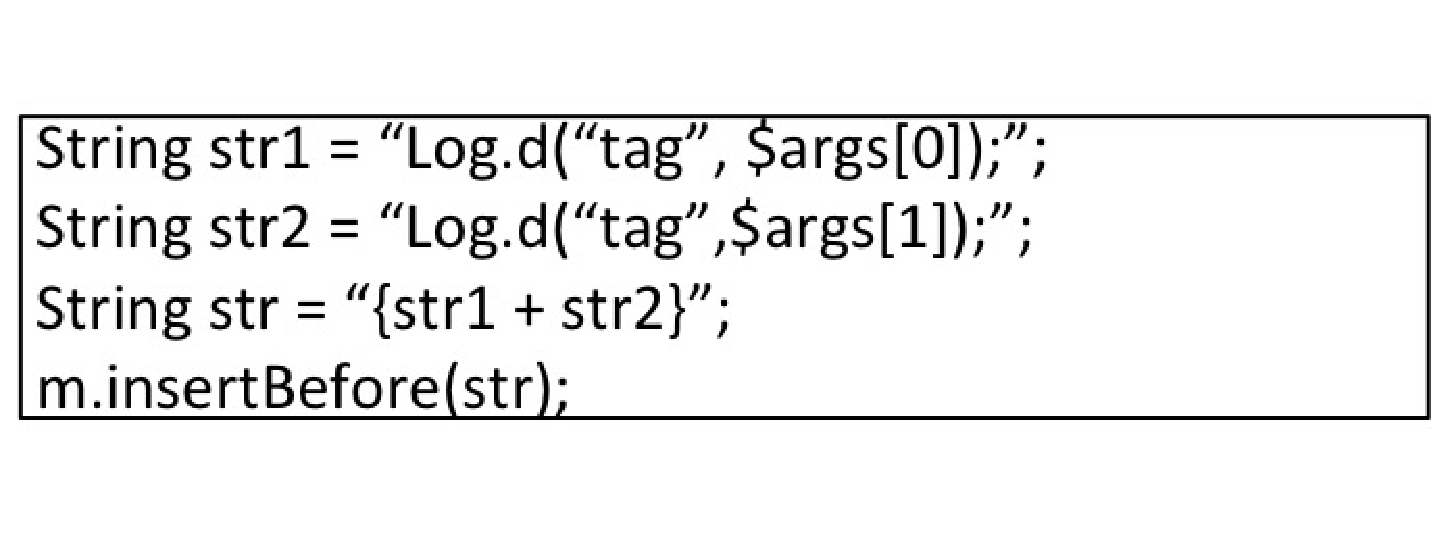
\includegraphics[scale=0.3]{insertbefore2.eps}
\end{center}
\caption{CtMethod.insertbefore の使用例}
\label{insertbefore}
\end{figure}


\begin{figure}[t]
\begin{center}
\graphicspath{{./epsfiles/}}
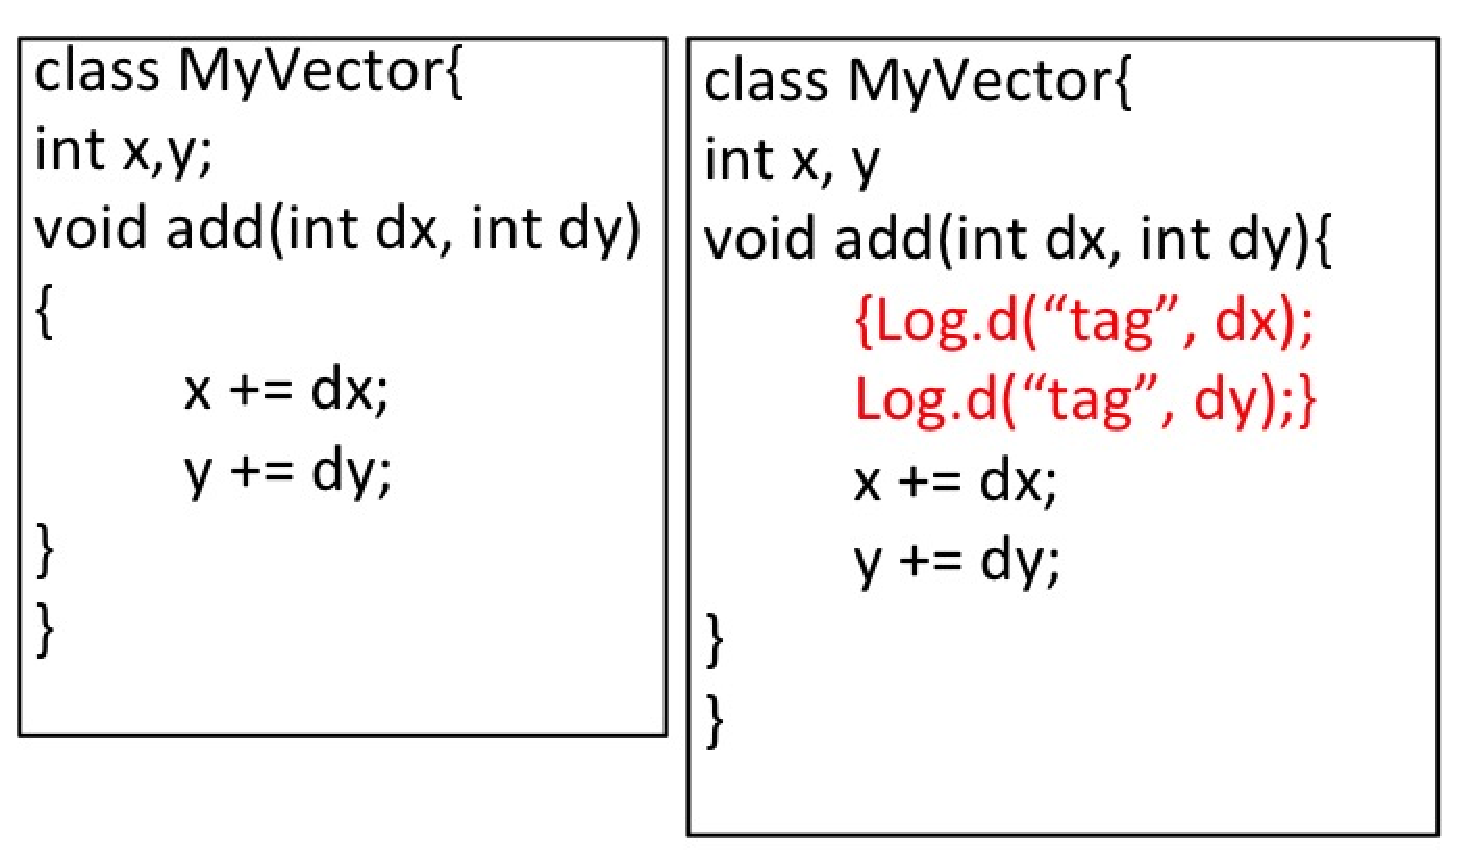
\includegraphics[scale=0.3]{vector.eps}
\end{center}
\caption{insertBefore 実行前後の MyVector クラス}
\label{vector}
\end{figure}

\subsubsection{メソッド呼び出しの置き換え}
\label{replacement}
\ref{methodcalls} の提案を実現するために,メソッドの置き換えを行う.
\ref{methodcalls} では,メソッドの前後にコードを挿入すると述べたが,この場合には,\ref{insertcodes} で説明した insertBefore を用いることはできない.
なぜなら,この場合はメソッドの先頭ではなく,それぞれのメソッド呼び出しの前後にコードを挿入するためである.
そのため, コードの置き換えを行う別のメソッドを用いる.

 Javassist のメソッドの replace によりメソッド呼び出しの置き換えを行う.
図\ref{replace}はこのメソッドの使用例である.
図中の m はメソッド呼び出しを表すオブジェクト (javassist.expr.MethodCall) である.
ある methodA の中の method1 が m だったとすると,図\ref{methoda}のようになる
"\$\_= \$proceed(\$\$);" は置換される元のコードを実行する文である.
\$, \$proceed, \$\$ も \$args と同様,Javassist の特殊変数である.
\$\_ は置換される元のコードの計算結果,\$proceed は置換される前の呼び出されるメソッド名 (図  では method1 となる), \$\$ は元のメソッド呼び出し式の引数列を表す.

メソッド呼び出しの前後に入るログコードには,次に示す情報を出力させるコードである.
1. 呼び出されるメソッドの名前,2. そのメソッドのクラス,3. 返り値の型,4. 引数の型,5. 呼び出しているメソッド名,を含んだ文字列を作る.
この文字列を図\ref{replace}の str1 の "before", str3 の "after" にあたる場所へ代入する.
これらの情報は Javassist の API を用いることで取得できる.

メソッド呼び出しを置き換えるプログラムの全体の流れは\ref{insertcodes}と同様である.
前処理として,コードを挿入するクラスを決定する.
そして,入力されたクラスを検索し,見つかったクラスのそれぞれのメソッドに対して先に述べた replace による置き換えを行う.

\begin{figure}[t]
\begin{center}
\graphicspath{{./epsfiles/}}
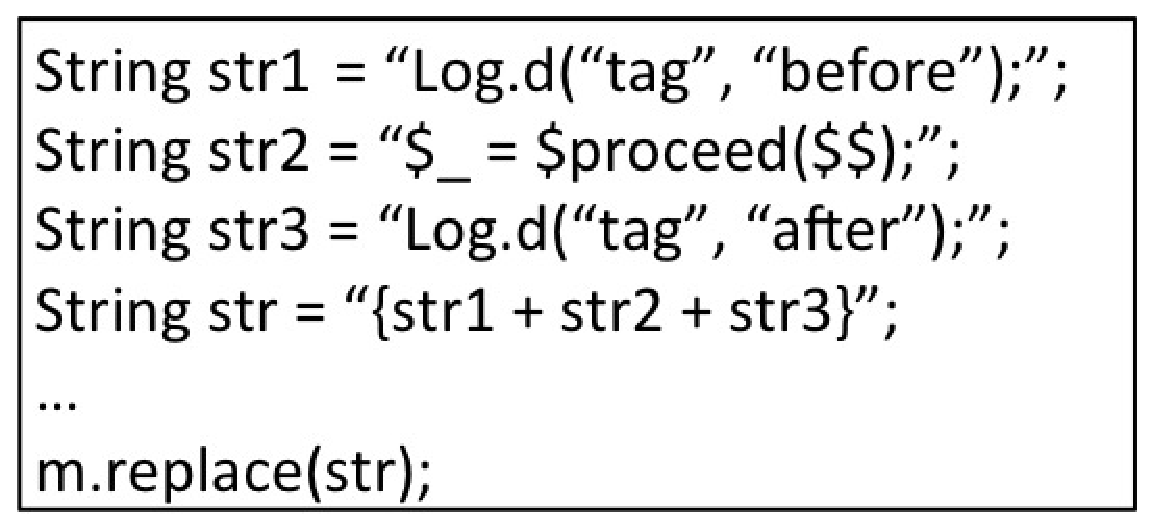
\includegraphics[scale=0.3]{replace.eps}
\end{center}
\caption{MethodCall.replace の使用例}
\label{replace}
\end{figure}

\begin{figure}[t]
\begin{center}
\graphicspath{{./epsfiles/}}
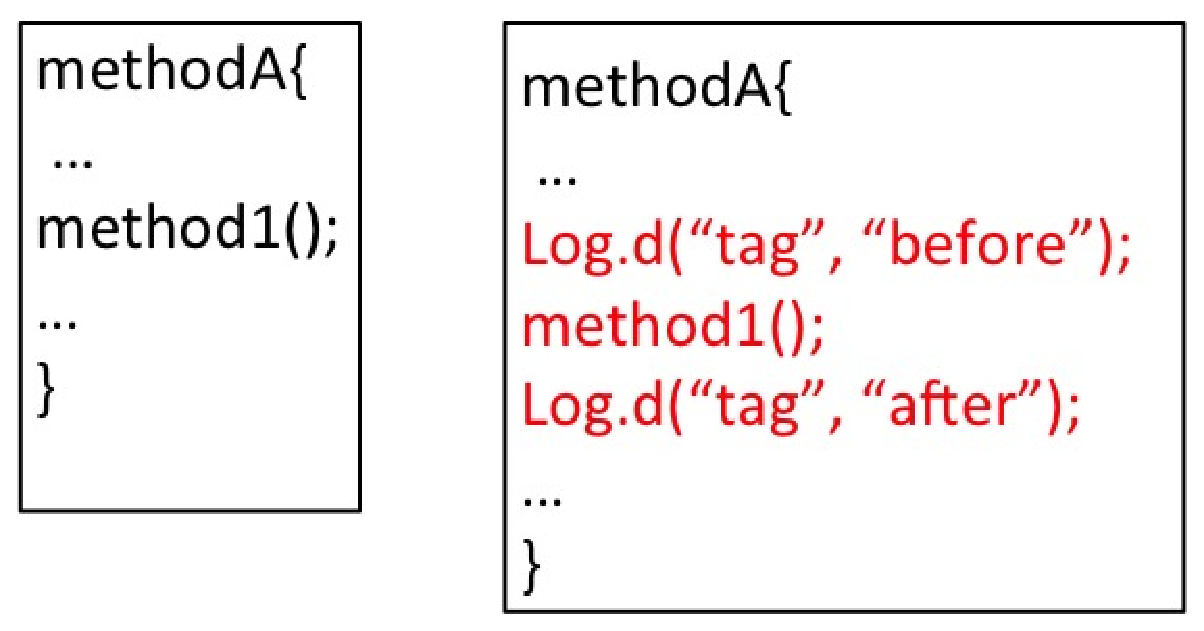
\includegraphics[scale=0.3]{methoda.eps}
\end{center}
\caption{replace 実行前後の metthodA メソッド}
\label{methoda}
\end{figure}

\subsubsection{private メソッドを書き換える方法}
\label{private}
\ref{insertcodes} で 
private メソッドにコードを挿入する方法は public メソッドとは異なる.
Javassist の中で,クラスを表すオブジェクト javassist.CtClass がある.
CtClass のメソッド getMethods はそのクラスが持つメソッド (CtMethod) の配列を返す.
しかし,private メソッドは getMethods の返り値の配列には入らない仕様となっている.
\ref{insertcodes}, \ref{replacement} では,getMethods で返されたメソッドのみに対してコードを挿入した.
より詳細なログを得るためには private メソッドを書き換える必要がある.

この解決策は,\ref{replacement}のプログラムで得たログからprivate メソッド名とそのクラス名を取得することだ.
\ref{replacement}のプログラムでは,private メソッドの前後にもログを挿入することが可能である.
メソッド名とそのクラス名がわかっていれば,そのメソッドのアクセス修飾子を変えることができる.
この場合,CtMethod オブジェクトを自分で宣言することができるため,getMethods を用いることなく,CtMethod オブジェクトを得ることができる. 
よって,CtMethod クラスのメソッドである,setModifier を用いて private から public に変えることができる.

なお,もともと private であったメソッドを public にした場合,private に戻す必要がある.
public にしたままで Android の実機で実行したところ,インストールはできたが,アプリを実行できなかった.
この時に Android OS が出したログには,実行が失敗した原因は private なメソッドが public になっているためと説明されていた.
そのため,private から public にしたメソッドを元に戻した(private に戻して) ところ,正常に動作した.

\subsection{得られたログを処理するためのプログラム}
\label{splitscript}
目的

比較

\begin{itembox}[c]{DDMS より得られたログの一部}
\footnotesize{
%\begin{verbatimtab}[4]
12-17 15:07:40.063: D/(12568): CLASS: com.mj.iMatch.IMatch METHOD: onCreate args[0]:android.os.Bundle = null\\
12-17 15:07:40.063: D/(12568): ID: 321 Before onCreate Called From onCreate In com.mj.iMatch.IMatch\\
12-17 15:07:40.063: D/(12568): ID: 321 After onCreate Backed To onCreate In com.mj.iMatch.IMatch\\
...\\
12-17 15:07:40.063: D/(12568): ID: 55 After getDefaultDisplay Backed To  onCreate In com.mj.iMatch.IMatch\\
12-17 15:07:40.063: D/(12568): CLASS: com.mj.iMatch.CommonUtils METHOD: setDisplay args[0]:android.view.Display = Display id 0: DisplayInfo{"Built-in Screen", app 1080 x 1776, real 1080 x 1920, largest app 1794 x 1701, smallest app 1080 x 1005, 60.0 fps, rotation0, density 480 (442.451 x 443.345) dpi, layerStack 0, type BUILT\_IN, FLAG\_SECURE, FLAG\_SUPPORTS\_PROTECTED\_BUFFERS}, DisplayMetrics{density=1.0, width=320, height=526, scaledDensity=1.0, xdpi=147.48367, ydpi=147.78168}, isValid=true\\
12-17 15:07:40.063: D/(12568): ID: 688 Before getWidth Called From setDisplay In com.mj.iMatch.CommonUtils\\
12-17 15:07:40.063: D/(12568): ID: 688 After getWidth Backed To  setDisplay In com.mj.iMatch.CommonUtils\\
12-17 15:07:40.063: D/(12568): ID: 741 Before getHeight Called From setDisplay In com.mj.iMatch.CommonUtils\\
12-17 15:07:40.063: D/(12568): ID: 741 After getHeight Backed To  setDisplay In com.mj.iMatch.CommonUtils\\
12-17 15:07:40.083: D/(12568): ID: 184 Before setContentView Called From onCreate In com.mj.iMatch.IMatch\\
12-17 15:07:40.133: D/(12568): CLASS: com.admob.android.ads.AdManager METHOD: isEmulator args[]: No Parameter\\
12-17 15:07:40.133: D/(12568): ID: 647 Before equals Called From isEmulator In com.admob.android.ads.AdManager\\
12-17 15:07:40.133: D/(12568): ID: 647 After equals Backed To  isEmulator In com.admob.android.ads.AdManager\\
....\\
12-17 15:07:40.183: D/(12568): ID: 455 Before loadPreferences Called From onResume In com.mj.iMatch.IMatch\\
12-17 15:07:40.183: D/(12568): CLASS: com.mj.iMatch.IMatch METHOD: loadPreferences args[]: No Parameter\\
12-17 15:07:40.183: D/(12568): ID: 12 Before getSharedPreferences Called From loadPreferences In com.mj.iMatch.IMatch\\
12-17 15:07:40.183: D/(12568): ID: 12 After getSharedPreferences Backed To  loadPreferences In com.mj.iMatch.IMatch\\
12-17 15:07:40.183: D/(12568): ID: 667 Before getInt Called From loadPreferences In com.mj.iMatch.IMatch\\
12-17 15:07:40.183: D/(12568): ID: 667 After getInt Backed To  loadPreferences In com.mj.iMatch.IMatch\\
12-17 15:07:40.183: D/(12568): ID: 455 After loadPreferences Backed To  onResume In com.mj.iMatch.IMatch\\
%\end{verbatimtab}
}
\end{itembox}


\begin{itembox}[c]{クラスごとに分けたログの一部}
\footnotesize{
\begin{verbatimtab}[4]
0 CLASS com.mj.iMatch.IMatch METHOD onCreate args[0]android.os.Bundle = null
1	 ID 321 Before onCreate Called From onCreate In com.mj.iMatch.IMatch
2	 ID 321 After onCreate Backed To  onCreate In com.mj.iMatch.IMatch
...
76	 ID 455 Before loadPreferences Called From onResume In com.mj.iMatch.IMatch
77	 CLASS com.mj.iMatch.IMatch METHOD loadPreferences args[] No Parameter
78		 ID 12 Before getSharedPreferences Called From loadPreferences 
In com.mj.iMatch.IMatch
79		 ID 12 After getSharedPreferences Backed To  loadPreferences 
In com.mj.iMatch.IMatch
80		 ID 667 Before getInt Called From loadPreferences In com.mj.iMatch.IMatch
81		 ID 667 After getInt Backed To  loadPreferences In com.mj.iMatch.IMatch
82	 ID 455 After loadPreferences Backed To  onResume In com.mj.iMatch.IMatch

\end{verbatimtab}
}
\end{itembox}
